% !TEX program lualatex
\documentclass{EU-report}
\usepackage{longtable}
\usepackage[style=verbose-trad1,bibstyle=eubibstyle,sorting=none,maxbibnames=100,firstinits=true,backend=bibtex]{biblatex}

\bibliography{references-Groningen,utz-collection,science-tlp}

\graphicspath{{./}{./Figures/}{../Figures/}}

\begin{document}

\begin{center}
\vfill
Project Number: 737043\\[1cm]
Project Acronym: \textbf{TISuMR}\\[1cm]
Project Title: \textbf{Integrated Tissue Slice Culture and NMR Metabolomics
  --- A Novel Approach Towards Systemic Understanding of Liver Function And Disease}\\
\vfill
{\Huge TISuMR Device Specification\\}
\vfill

\includegraphics[width=5cm]{tisumr-logo-small}
\end{center}
\vfill
Document version: 0.0.0 \\
Last modified: \today
\vspace{1cm}

\clearpage
\section{Executive Summary}

\section{Change History}
\begin{center}
	\begin{tabular}{lrp{7cm}r} \hline\hline
		\emph{Version} & \emph{Mod. Date} & \emph{Summary of changes} & \emph{Author} \\
		\hline
		0.0.0 & 22/5/2019 & Initial discussion version & ms, mu\\
		\hline\hline
	\end{tabular}
\end{center}
\clearpage

% ========== Edit your name here
%\author{}
%\title{TISuMR device specifications}
%\maketitle

%\medskip
\section{Scope of this document}
TISuMR is a collaboration project between University of Southampton, University
of Groningen and Karlsruhe Institute of Technology. The aim of the project is to
develop technologies for NMR (nuclear magnetic resonance) compatible
microfluidic perfusion culture of PCLS (precision cut liver slices).
The devices that are being developed at the three project partner sites
are built for different aims (high-resolution liquid NMR spectroscopy of the
perfusion fluid, high-resolution magic-angle spinning NMR spectroscopy,
or conventional analysis using HPLC and other techniques). These different
approaches lead to different interfacing requirements for the perfusion system.
In order to ensure comparability of the results, it is necessary to standardise
certain aspects of the design. This will ensure identical culture conditions,
as well as a common standard to judge the performance of the culture
system and basic viability of the tissue slices.

This document defines the specifications for a device design to be qualified as
a TISuMR device. All the TISuMR personnel will follow these requirements for
device design if the device is used for TISuMR research. Possible variations are
also given to cater to specific experimental needs.

Changes to this document will be decided in the TISuMR meetings. The intended
changes will be communicated to all the partners before the meeting to think
upon. All the partners should agree for a change to be made final. This document
will be available on
\url{https://github.com/marcel-utz/tisumr-device} to obtain the latest version
of the document. Marcel Utz will own the master copy and will be responsible to
implement the changes. A drawing of the proposed device is shown in
Fig.\ref{fig:tisumr-device}

\section{Required Specifications}
\begin{itemize}
\item \textbf{Culture chamber geometry:} The culture chamber is cylindrical in
shape with a diameter of 7$\pm$1 mm and a depth of 500$\pm$100 $\mu$m.
%The overall thickness of the device is less than 1 mm.
% mu: I suggest removing this, as it is not essential.
\item \textbf{Perfusion geometry:} The perfusion fluid flows around the PCLS.
There can be more than one inlets and outlets. The inlet and outlet channels
have cross sectional dimensions of 200$\pm$100$\times$200$\pm$100 $\mu$m$^2$.
\item \textbf{Chip or device material:} Polycarbonate is used for the chip or
device fabrication.
\item \textbf{Temperature:}. The PCLS culture is performed at
37$\pm$0.5 $^{\circ}$C.
\item \textbf{Gas composition:} Either carbogen (95 \% O$_2$ + 5 \% CO$_2$) or a mixture (80 \% O$_2$+ 10 \% N$_2$ +5 \% CO$_2$) is used
for the culture. Gas composition with 70 \% or more O$_2$ partial pressure have the same effect on viability of PCLS.
\item \textbf{Viability standards:} Adenosine tri(phosphate) (ATP) content in
the tissue slice after culture is used as a measure of viability. As a rule,
tissue slices can be considered viable if they contain at least 6~pmol of ATP
per mg of protein. The protocols for ATP determination is given in section\ref{atp} and for protein determination is given in section\ref{protein}.
\item \textbf{Medium composition:} William E  with Glutamax + Glucose (1.375
g/500mL William E medium) + Gentamycine (500$\mu$L/500mL)
\item \textbf{Sterilization:} Sterilisation will be preformed by exposure of the equipment to 70\% ethanol in water for 5 minutes and drying them afterwards. Tubings will be sterilised by flowing 70\% ethanol in water for half an hour and then flow phosphate-buffered saline (PBS) for a wash.
\end{itemize}

\section{Allowed variations}
\begin{itemize}
\item \textbf{Detailed fluidic paths:} Fluidic network can be designed freely.
\item \textbf{Flow protocol:} The media can be flowed by different types of
pumps or centrifuge.
\item \textbf{Fabrication method:} The devices can be made through machining or
bonding layers by different protocols.
\item \textbf{Flow rates:} Range of flow rates will be decided through
optimisation.
\item \textbf{LDH:} If ATP content can not be measured due to the nature of experiment, LDH (lactate dehydrogenase) can be used as a viability indicator.
\end{itemize}

\begin{figure}
\centering

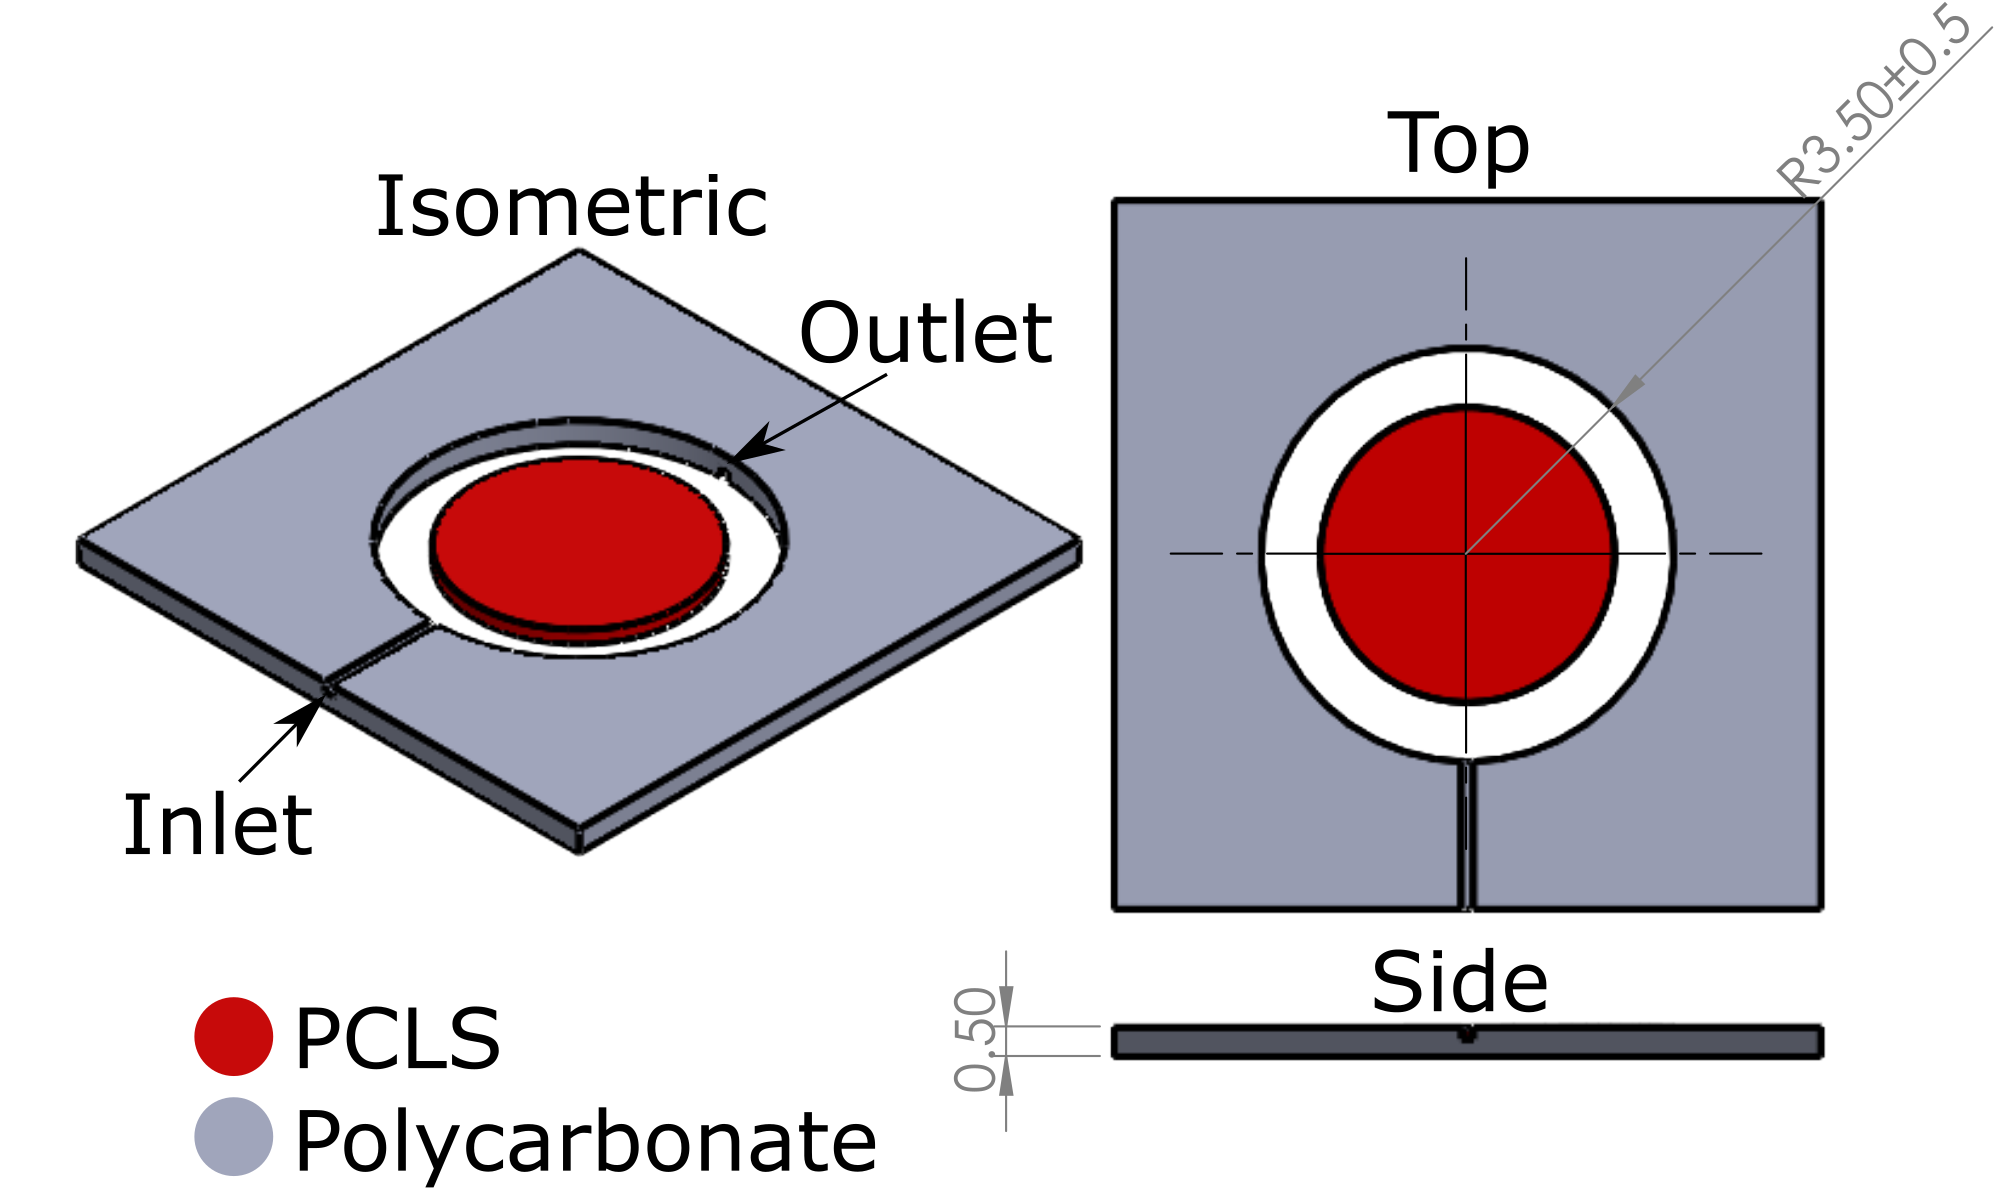
\includegraphics[width=.8\linewidth,keepaspectratio=true]{./device/tisumr-device.png}
\caption{Isometric, top and side views of the device. The diameter of the PCLS
chamber is 0.7 mm. The thickness of the chamber is 0.5 mm.}
\label{fig:tisumr-device}
\end{figure}

\section{ATP determination}
\label{atp}
\begin{itemize}
%\item \textbf{Goal:} Assay to determine the ATP levels in tissue slices.
\item \textbf{Materials:}
\begin{itemize}
\item 1.5mL tubes
\item White 96-wells plate
\item Minibead-beater
\item Repetitive pipet with 50 $\mu$l tip
\item Synergy HT plate reader
\item ATP positive control (P) (-80 $^{\circ}$C) (1 aliquot/plate)
\end{itemize}
\item \textbf{Solutions}
\begin{itemize}
\item \textbf{SONOP (Sonification Solution), Ethanol (70\% v/v) containing 2mM EDTA (M=372.24 g/mol) with pH=10.9}
For 1L: Dissolve 0.744g EDTA in $\pm$ 200ml of MQ-water, adjust pH with 5M NaOH to pH=10.9, add 60mL MQ-water and 740ml ethanol (96\%)
\item \textbf{100mM Tris-HCl, 2mM EDTA buffer (pH 7.6-8.0)} For 500ml: Dissolve 6.0g Tris (M=121.14) (Tris(hydroxymethyl)amniophen; Merck) and 0.37g EDTA (Triplex III; M=372.24) in $\pm$ 300ml MQ-water, adjust pH with 6N HCl and fill up to 500ml total volume with MQ-water.
\item \textbf{ATP Bioluminescence assay kit Roche.}
\begin{itemize}
\item Luciferase reagent lyophilized (white cap):
Dissolve lyophilized luciferase in exactly 10.0 ml MQ-water and mix by swinging. Do not vortex.
\item ATP-standard $\pm$ 10mg lyophilized (red cap):
 Dissolve the ATP-standard from the kit to exactly 10mg/ml (= 16.5mM) with MQ-water) and aliqoute 20 $\mu$L and store in -80 $^{\circ}$C
\end{itemize}
\end{itemize}
\item \textbf{Protocol}:After the incubation put 1 slice in 1 ml SONOP in a safelock vial, 1 cup of minibead and snap frozen in liquid N$_2$.
\begin{enumerate}
\item Label a new set of 1.5mL tubes (equal to the amount of ATP-samples).
\item Get luciferase from fridge or freezer, this needs to be at room temperature.
\item Homogenize the sample with minibead-beater for \textbf{2$\times$45sec}. Store the samples back on ice.
\item Centrifuge homogenate \textbf{5min at 13.000 rpm at 4 $^{\circ}$C}. Transfer the supernatant into the new tube and \textbf{keep on ice}. The tube with precipitate is dried at 37 $^{\circ}$C (1 day) or at RT (3 days) for protein measurement.
\item Prepare a calibration curve and store tubes on ice:
\begin{center}
	\begin{tabular}{lrp{7cm}r} \hline\hline
\textbf{Dilution} & \textbf{Amount ($\mu$l)} 	 & \textbf{ Tris/EDTA Buffer ($\mu$l)} & \textbf{ Conc. (M)} \\
\hline
 \textbf{A}	 	& 10$\mu$l ATP-standard (S)	& 90							& 1.65$\times$ 10$^{-3}$\\
 \hline
 \textbf{B}	 	& 50$\mu$l [A]				 & 450						& 1.65 $\times$ 10$^{-4}$\\
 \hline
 \textbf{C}	 	& 50$\mu$l [B]			 	& 450						& 1.65 $\times$ 10$^{-5}$\\
 \hline
 \textbf{Cal 1}	&  50$\mu$l [C]			   	& 450						& 1.65 $\times$10$^{-6}$\\
 \hline
 \textbf{Cal 2}	& \textbf{100$\mu$l [Cal 1]!}	& \textbf{400}					& 3.30 $\times$ 10$^{-7}$\\
 \hline
 \textbf{Cal 3}	& 50$\mu$l [Cal 1]!	 	  	& 450						& 1.65 $\times$ 10$^{-7}$\\
 \hline
 \textbf{Cal 4}	& \textbf{100$\mu$l [Cal 3]!}	& \textbf{400}					& 3.30 $\times$ 10$^{-8}$\\
 \hline
 \textbf{Cal 5}	& 50$\mu$l [Cal 3]!			& 450						& 1.65 $\times$ 10$^{-8}$\\
\hline
	\end{tabular}
\end{center}
\item Pipet 5$\mu$l Blank (Tris/EDTA), 5$\mu$l positive control, and 5$\mu$L supernatant of each sample in duplo to the white 96-wells plate.
\item Add 45$\mu$l Tris/EDTA buffer to all wells containing blank, positive control or sample. 
\item Pipette 50$\mu$l diluted calibration curve in duplo in the plate.
\item Add 50$\mu$l luciferase (do not vortex) to every well using a repetitive pipet or a multichannel pipet.
\item Shake plate a little and measure plate after 0min, 5min and 10 min using the luminometer (set-up SynergyHT ATP protocol, kinetic read (3 timepoints interval 5 min) for luminenscence).
\end{enumerate}
\item \textbf{Remarks:} Important: The ATP in the slices is sensitive for breakdown by present enzymes. Therefore store samples at -80 $^{\circ}$C and keep tubes at 4$^{\circ}$C throughout the determination.
\end{itemize}

\section{Protein determination}
\label{protein}
\begin{itemize}
\item \textbf{Materials:}
\begin{itemize} 
\item BSA stock solution 3.2 (A) and 2.4 (B) mg/mL
\item Water bath with shaking function
\item Minibead beater
\item Transparent flat 96-wells plate
\item Multichannel pipet
\item Protein reader absorbance at wavelength 650nm*
\end{itemize}
\item \textbf{Solutions:}
\begin{itemize}
\item 5M NaOH solution (20g sodium hydroxide/100mL)
\item Reagent A and B of BIO-rad kit.
\end{itemize}
\item\textbf{Protocol}:
\begin{enumerate}
\item Turn on waterbath 
\item Thaw BSA (3.2 and 2.4 mg/ml)
\item Add (to pellet and beads) 200 $\mu$l 5M NaOH (20g in 100ml)
\item Incubate 30 min at 37$^{\circ}$C (shaking, high speed) inside the waterbath
\item Make the following calibration curve diluted in the buffer at concentrations: 0 - 0.2 - 0.4 - 0.6 - 0.8 - 1.2 mg/ml
\begin{center}
	\begin{tabular}{lrp{7cm}r} \hline\hline
\textbf{Dilution} & \textbf{Amount ($\mu$l)} 	 & \textbf{ 1M NAOH ($\mu$l)} & \textbf{ Conc. (mg/ml)} \\
\hline
 \textbf{}	               &                                                               & 					                        & \\
 \hline
 \textbf{A1}	 	& 50$\mu$l [A]	                                        & 50							& 1.6\\
 \hline
 \textbf{A2}	 	& 50$\mu$l [A1]			              & 50						        & 0.8\\
 \hline
 \textbf{A3}	 	& 50$\mu$l [A2]			 	      & 50						       & 0.4\\
 \hline
 \textbf{A4}	       &  50$\mu$l [A3]			   	              & 50						       & 0.2\\
 \hline
 \textbf{A5}	       & 50$\mu$l [A4]	                                       & 50					               & 0.1\\
 \hline
 \textbf{A6}	       &                                                               & 50					               & 0.0\\
 \hline
 \textbf{}	               &                                                               & 					                        & \\
 \hline

 \textbf{B1}	      & 30$\mu$l [A] 	  	                               & 50					               & 1.2 \\
 \hline
 \textbf{B2}	      & 50$\mu$l [B1]                                          &50					              & 0.6\\
 \hline
 \textbf{B3}	      & 50$\mu$l [B2]		                               & 50						      & 0.3\\
\hline
	\end{tabular}
\end{center}
\item Add 800 $\mu$l milliQ water (5x dilution, same as volume in SONOP)
\item Homogenize again with minibeadbeater for 40 seconds
\item Pipette 5 $\mu$l of calibration standard or sample in 96 well clear plate.
\item Add 25 $\mu$l of reagent A in each well (standards and samples).(If samples contain detergent than 20 $\mu$l of reagent S is added to 1 ml of reagent A)
\item Add 200 $\mu$l of reagent B to each well (standards and samples).
\item Keep the plate for 15 minutes at room temperature and measure the absorbance at wavelengths 750 or 650* nm  (Stable for 1 hour)
\end{enumerate}
\item \textbf{Remarks:} With the Biorad reader, please use 655nm wavelength instead. 
\end{itemize}

\end{document}
